%!TEX program = xelatex
\documentclass[9pt, compress]{beamer}
\usetheme[titleprogressbar]{m}

\usepackage{array}
\usepackage{tabu}
\usepackage{longtable} %tabu needs this to be loaded.
\usepackage{lipsum}

\usepackage{rotating}

\usepackage{color}
\usepackage{xcolor}
\usepackage{listings}
\usepackage{sectsty}
\usepackage{caption}


\DeclareCaptionFont{white}{\color{white}}
\DeclareCaptionFormat{listing}{\colorbox{gray}{\parbox{\dimexpr\textwidth-1.72\fboxsep\relax}{#1#2#3}}}
\captionsetup[lstlisting]{format=listing,labelfont=white,textfont=white,margin=0pt}
\lstset{language=C,
	basicstyle=\footnotesize,
	keepspaces=true,
	tabsize=4,               
	frame=single,                           % Single frame around code
	rulecolor=\color{black},
	captionpos=b,
	showstringspaces=false,	
	abovecaptionskip=-0.9pt,
	xleftmargin=3.4pt,
	xrightmargin=2.6pt,
	breaklines=true,
	postbreak=\raisebox{0ex}[0ex][0ex]{\ensuremath{\color{black}\hookrightarrow\space}},
	xleftmargin=3.2pt,
	escapechar=\&,
	literate={а}{{\selectfont\char224}}1
	{~}{{\textasciitilde}}1
	{б}{{\selectfont\char225}}1
	{в}{{\selectfont\char226}}1
	{г}{{\selectfont\char227}}1
	{д}{{\selectfont\char228}}1
	{е}{{\selectfont\char229}}1
	{ё}{{\"e}}1
	{ж}{{\selectfont\char230}}1
	{з}{{\selectfont\char231}}1
	{и}{{\selectfont\char232}}1
	{й}{{\selectfont\char233}}1
	{к}{{\selectfont\char234}}1
	{л}{{\selectfont\char235}}1
	{м}{{\selectfont\char236}}1
	{н}{{\selectfont\char237}}1
	{о}{{\selectfont\char238}}1
	{п}{{\selectfont\char239}}1
	{р}{{\selectfont\char240}}1
	{с}{{\selectfont\char241}}1
	{т}{{\selectfont\char242}}1
	{у}{{\selectfont\char243}}1
	{ф}{{\selectfont\char244}}1
	{х}{{\selectfont\char245}}1
	{ц}{{\selectfont\char246}}1
	{ч}{{\selectfont\char247}}1
	{ш}{{\selectfont\char248}}1
	{щ}{{\selectfont\char249}}1
	{ъ}{{\selectfont\char250}}1
	{ы}{{\selectfont\char251}}1
	{ь}{{\selectfont\char252}}1
	{э}{{\selectfont\char253}}1
	{ю}{{\selectfont\char254}}1
	{я}{{\selectfont\char255}}1
	{А}{{\selectfont\char192}}1
	{Б}{{\selectfont\char193}}1
	{В}{{\selectfont\char194}}1
	{Г}{{\selectfont\char195}}1
	{Д}{{\selectfont\char196}}1
	{Е}{{\selectfont\char197}}1
	{Ё}{{\"E}}1
	{Ж}{{\selectfont\char198}}1
	{З}{{\selectfont\char199}}1
	{И}{{\selectfont\char200}}1
	{Й}{{\selectfont\char201}}1
	{К}{{\selectfont\char202}}1
	{Л}{{\selectfont\char203}}1
	{М}{{\selectfont\char204}}1
	{Н}{{\selectfont\char205}}1
	{О}{{\selectfont\char206}}1
	{П}{{\selectfont\char207}}1
	{Р}{{\selectfont\char208}}1
	{С}{{\selectfont\char209}}1
	{Т}{{\selectfont\char210}}1
	{У}{{\selectfont\char211}}1
	{Ф}{{\selectfont\char212}}1
	{Х}{{\selectfont\char213}}1
	{Ц}{{\selectfont\char214}}1
	{Ч}{{\selectfont\char215}}1
	{Ш}{{\selectfont\char216}}1
	{Щ}{{\selectfont\char217}}1
	{Ъ}{{\selectfont\char218}}1
	{Ы}{{\selectfont\char219}}1
	{Ь}{{\selectfont\char220}}1
	{Э}{{\selectfont\char221}}1
	{Ю}{{\selectfont\char222}}1
	{Я}{{\selectfont\char223}}1,
	extendedchars=true
}

%галочка
\usepackage{amssymb}% http://ctan.org/pkg/amssymb
\usepackage{pifont}% http://ctan.org/pkg/pifont
\newcommand{\cmark}{\ding{52}}%
\newcommand{\xmark}{\ding{56}}

\usepackage{booktabs}  
\usepackage[scale=2]{ccicons}
\usepackage{minted}
\usepgfplotslibrary{dateplot}
\usemintedstyle{trac}
\author{Студент: \textbf{Д.В. Круминьш}\\ 
	Группа: \textbf{13541/3}\\ \\
	Преподаватель: \textbf{И.А. Малышев} } 
\title{Отчет о лабораторной работе №2}
\subtitle{Курс: \textbf{Администрирование компьютерных сетей}\\
Тема: \textbf{Тестирование компьютерной сети на основе TCP/IP}}
%\logo{123}
\institute{Санкт-Петербургский политехнический университет Петра Великого}
\date{ }
%\subject{}
%\setbeamercovered{transparent}
%\setbeamertemplate{navigation symbols}{}
\begin{document}
	\maketitle
%	\begin{frame}
%		\frametitle{Оглавление}
%		\tableofcontents{}
	%\end{frame}
\begin{frame}
\frametitle{Цели работы}
\begin{enumerate}
\item Изучение утилит и систем администрирования TCP/IP-сетей.
\item Мониторинг и анализ характеристик TCP/IP-сетей.
\end{enumerate}
\end{frame}

\section{Оценка пропускной способности}
\begin{frame}
\frametitle{Утилита iperf}
\textbf{Iperf} — кроссплатформенная консольная клиент-серверная программа, предназначена для тестирования пропускной способности интернет канала между двумя компьютерами.\\\\
\textbf{Как работает}.\\
Измерение осуществляется следующим образом, на одном ПК запускаем iperf в режиме «сервер», на втором в режиме «клиент» с указанием ip-адреса первого ПК («сервера»). Через заданное время показывается измеренная информация.\\\\
В работе использовалась \textbf{версия} 2.0.5
\end{frame}

\begin{frame}[fragile]
\frametitle{Установка iperf}
На \textbf{NetBsd}, были выполнены команды:
\begin{enumerate}
\item Загрузка iperf
\begin{enumerate}
\item Подключение к ftp серверу, к папке с пакетами для моей версии NetBSD
\begin{lstlisting}[language={}]
ftp -i ftp://ftp.netbsd.org/pub/pkgsrc/packages/NetBSD/x86_64/7.1.1/All/
\end{lstlisting}
\item Загрузка последней версии
\begin{lstlisting}[language={}]
mget iperf-2.0.5nb1.tgz
\end{lstlisting}
\item Завершение работы ftp
\begin{lstlisting}[language={}]
quit
\end{lstlisting}
\end{enumerate}
\item Создаем папку и разархивируем туда архив
\begin{lstlisting}[language={}]
mkdir iperf
tar -xzf iperf-2.0.5nb1.tgz -C /root/iperf
\end{lstlisting}
\item Утилита для запуска находится по пути \textbf{/root/iperf/bin}
\end{enumerate}
\end{frame}


\begin{frame}[fragile]
\frametitle{Установка iperf}
На \textbf{FreeBSD}, выполнены команды:
\begin{lstlisting}[language={}]
cd /usr/ports/benchmarks/iperf
make install clean
\end{lstlisting}
На \textbf{Kali Linux}, выполнена команда:
\begin{lstlisting}[language={}]
apt-get install iperf
\end{lstlisting}
На \textbf{Windows XP} скачены бинарные файлы программы.
\end{frame}

\begin{frame}[fragile]
\frametitle{Оценка пропускной способности используя iperf}
На хосте с FreeBSD запущен сервер iperf
\begin{lstlisting}[language={}]
iperf -s
\end{lstlisting}
На машинах(Kali Linux, NetBSD, Windows XP) iperf запущен в качестве клиента, командой:
\begin{lstlisting}[language={}]
iperf -c 192.168.40.2
\end{lstlisting}
В результате получены следующие данные:
\tabulinesep = 1mm
\begin{longtabu} to \textwidth {|X[ c , m ] |X[c , m ] | X[ c , m ]|}\firsthline\hline
\textbf{NetBSD}&\textbf{Kali Linux}&\textbf{Windows XP}\\ \hline \endfirsthead
1.47 Гбит/c&1.62 Гбит/c&5.81 Мбит/c\\ \hline
\end{longtabu}
\end{frame}


\section{Карта сети}

\begin{frame}[fragile]
\frametitle{Утилита 10-Страйк: Схема Сети}
Для изучения сети использована программа \textbf{10-Страйк: Схема Сети}(версия 3.32), установленная на Windows XP.

\begin{enumerate}
\item При запуске программы, были указаны диапазоны для сканирования;
\item Программа вывела список найденных хостов;
\item Была составлена карта сети.
\end{enumerate}
\end{frame}


\begin{frame}[fragile]
\frametitle{Указание диапазонов для сканирования}
\begin{center}  
	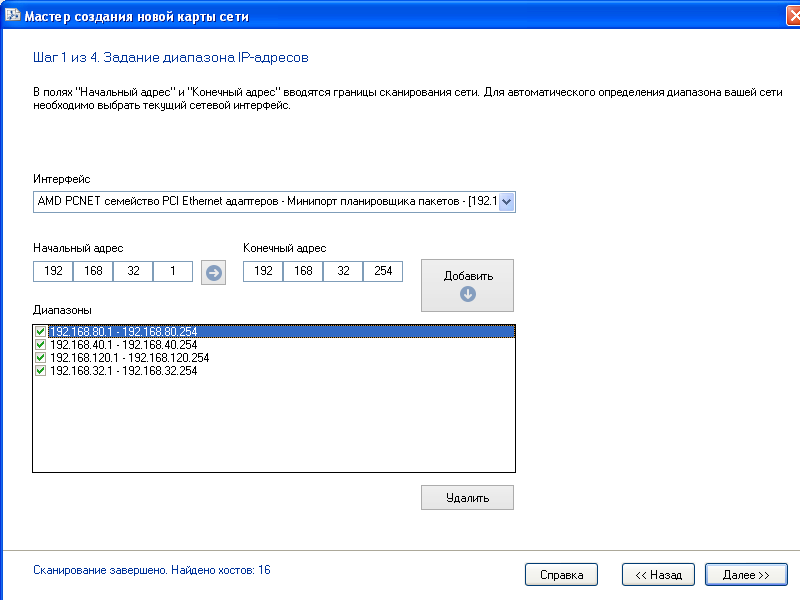
\includegraphics[width=.9\textwidth]{img/1}
\end{center}
\end{frame}

\begin{frame}[fragile]
\frametitle{Найденные хосты}
\begin{center}  
	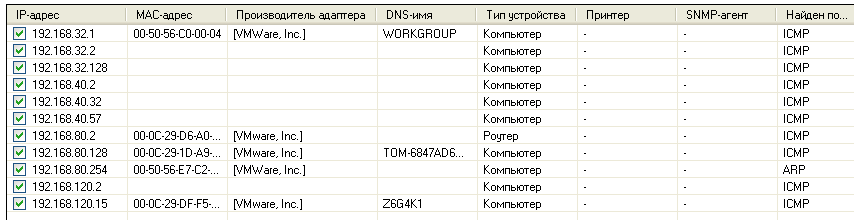
\includegraphics[width=\textwidth]{img/2}
\end{center}
\end{frame}

\begin{frame}[fragile]
\frametitle{Карта сети}
Программа не смогла определить точную карту сети, типы операционных систем, она видит лишь ближайший маршрутизатор, в данном случае – это FreeBSD (хост 192.168.80.2).
\begin{center}  
	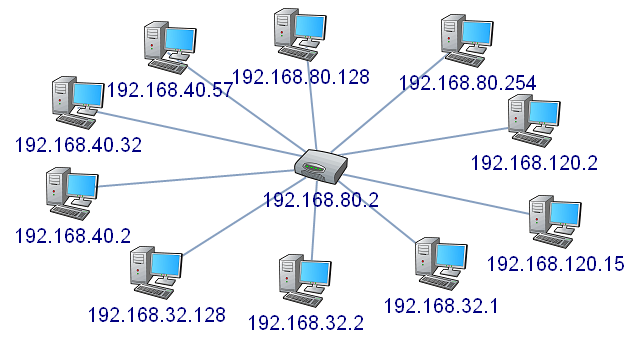
\includegraphics[width=.8\textwidth]{img/3}
\end{center}
\end{frame}

\section{Поиск уязвимостей}

\begin{frame}[fragile]
\frametitle{Утилита X-Spider}
В качестве программы по поиску уязвимостей была выбрана \textbf{X-Spider}(версия 7.7), которая была установлена на Windows XP.

Перед сканированием были добавлены следующие адреса интерфейсов:
\begin{itemize}
\item 192.168.80.128(Windwos XP);
\item 192.168.40.2(FreeBSD);
\item 192.168.80.2(FreeBSD);
\item 192.168.120.2(FreeBSD);
\item 192.168.120.15(Windows 98);
\item 192.168.40.32(Kali Linux);
\item 192.168.40.57(NetBSD);
\item 192.168.32.128(NetBSD);
\end{itemize}
\end{frame}


\begin{frame}
\frametitle{Найденные уязвимости}
\begin{center}  
	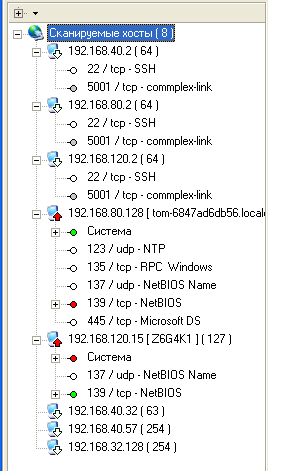
\includegraphics[width=.35\textwidth]{img/5}
	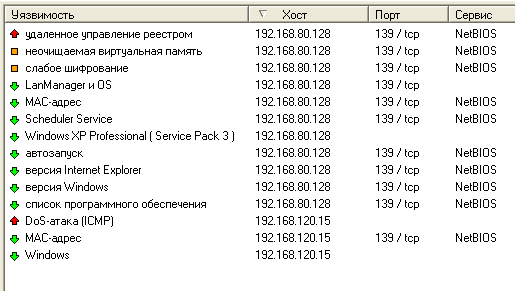
\includegraphics[width=.63\textwidth]{img/6}
\end{center}
\end{frame}


\begin{frame}
\frametitle{Найденные уязвимости}
Были выявлены следующие уязвимости:
\begin{itemize}
\item Windows XP
\begin{itemize}
\item имя операционной системе;
\item сервисом NTP открыт порт 123 по UDP;
\item сервисом RPC Windows открыт порт 135 по TCP;
\item сервисом NBNS открыт порт 137 по UDP;
\item сервисом NetBIOS открыт порт 139 по TCP.
\end{itemize}
\item Windows 98
\begin{itemize}
\item имя операционной системе;
\item сервисом NetBIOS-SSN открыт порт 137 по UDP;
\item сервисом NetBIOS открыт порт 139 по TCP.
\end{itemize}
\end{itemize}
В системах unix слабых мест не обнаружено.
\end{frame}


\begin{frame}[fragile]
\frametitle{Вывод}
В результате выполнения данной лабораторной работы была протестирована сеть на основе TCP/IP. 

Оценка пропускной способности показала свехвысокую скорость для ос семейства unix и весьма медленную для windows xp. Возможно это связано с кроссплатформенностью утилиты для тестирования и различных настроек операционных систем.

Утилита для построения карты сети, показала некорректную карту сети, что о говорит о сложности построения реальной карты сети.

Тестирование на уязвимости показало, что уязвимостям подвержены ОС семейства Windows, в то время как на unix системах уязвимостей найдено не было.


% про антивирус


\end{frame}	
	

	
\end{document}
